\documentclass{article}
\usepackage{../cs170}
\usepackage{pgfplots}
\pgfplotsset{compat=1.18}
\AtBeginDocument{\RenewCommandCopy\qty\SI}

\def\title{HW 01}

\begin{document}

\maketitle

\question{}

\begin{center}
    \begin{circuitikz}
        \draw (0, 2) to[V_=\(V_0\)] (0, 0) to[short] (4, 0) to[C, l_=\(C\)] (4, 2) to[R, l_=\(R\)] (2, 2) to[switch, l=\(s_1\), mirror, invert] (0, 2)
    ;\end{circuitikz}
\end{center}

The initial condition is \(V_C(t) = 0\).
Analyzing the current \(I_C(t)\),
\begin{align}
    \frac{V_0 - V_C(t)}{R} &= C \dv{V_C}{t} \\
    V_0 - V_C(t) &= RC \dv{V_C}{t} \\
    \frac{1}{V_0 - V_C(t)} &= \frac{1}{RC} \dv{t}{V_C} \\
    \int \frac{1}{V_0 - V_C(t)} \, \dd{V_C} &= \int \frac{1}{RC} \, \dd{t} \\
    -\ln|V_0 - V_C(t)| + C_0 &= \frac{t}{RC} + C_1 \\
    V_0 - V_C(t) &= C_2 e^{-\frac{t}{RC}} \\
    V_C(t) &= V_0 - C_2 e^{-\frac{t}{RC}}
\end{align}
Solving for the initial condition,
\begin{equation}
    0 = V_0 - C_2 \implies C_2 = V_0
\end{equation}
Thus, we have
\begin{align}
    V_C(t) &= V_0 (1 - e^{-\frac{t}{RC}}) \\
    I_C(t) &= C \dv{V_C}{t} = \frac{\cancel{V_0} - \cancel{V_0} + V_0 e^{-\frac{t}{RC}}}{R} = \frac{V_0}{R} e^{-\frac{t}{RC}}
\end{align}
Assuming \(V_0 = \qty{1}{\volt}\), \(R = \qty{1}{\ohm}\), and \(C = \qty{1}{\farad}\),
\begin{center}
    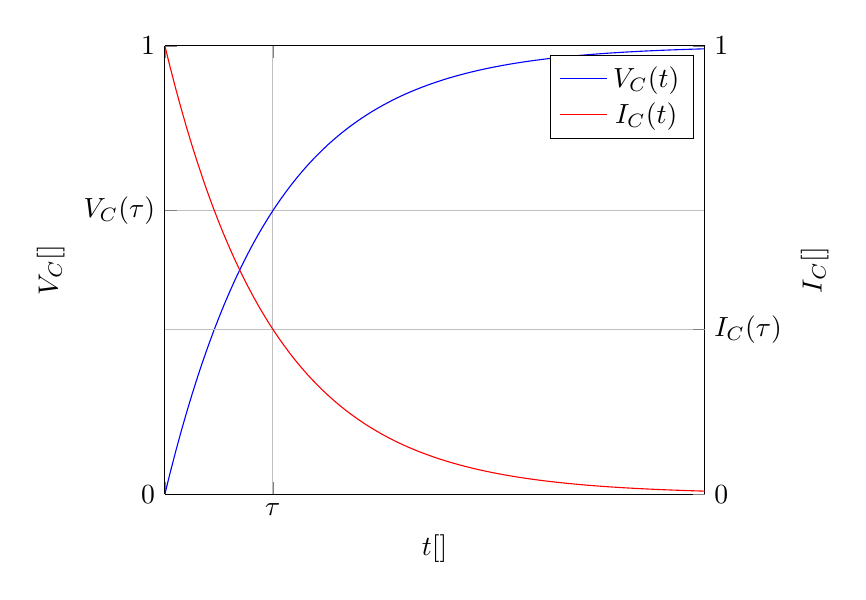
\begin{tikzpicture}
        \begin{axis}[
            axis y line*=left,
            xlabel = {\(t [\unit{\second}]\)},
            xticklabels={,,},
            ylabel = {\(V_C [\unit{\volt}]\)},
            xmin = 0, xmax = 5,
            ymin = 0, ymax = 1,
            xtick = {0, 1}, ytick = {0, 1},
            extra tick style = {grid=major},
            extra x ticks = {1},
            extra x tick labels = {\(\tau\)},
            extra y ticks = {1 - exp(-1)},
            extra y tick labels = {\(V_C(\tau)\)},
        ]
            \addplot[
            domain = 0:5,
            samples = 100,
            color = blue
            ]
            {1 - exp(-x)};
        \end{axis}

        \begin{axis}[
            axis y line*=right,
            axis x line = none,
            ylabel = {\(I_C [\unit{\ampere}]\)},
            ylabel near ticks, yticklabel pos=right,
            xmin = 0, xmax = 5,
            ymin = 0, ymax = 1,
            xtick = {0, 1}, ytick = {0, 1},
            extra tick style = {grid=major},
            extra y ticks = {exp(-1)},
            extra y tick labels = {\(I_C(\tau)\)},
        ]
            \addlegendimage{color=blue}\addlegendentry{\(V_C(t)\)}
            \addplot[
            domain = 0:5,
            samples = 100,
            color = red
            ]
            {exp(-x)};
            \addlegendimage{color=red}\addlegendentry{\(I_C(t)\)}
        \end{axis}
    \end{tikzpicture}
\end{center}

\question{}

\begin{center}
    \begin{circuitikz}
        \draw (0, 2) to[V_=\(V_0\)] (0, 0) to[short] (4, 0) to[L, l_=\(L\), mirror] (4, 2) to[R, l_=\(R\)] (2, 2) to[switch, l=\(s_1\), mirror, invert] (0, 2)
    ;\end{circuitikz}
\end{center}

The initial condition is \(I_L(t) = 0\).
Analyzing the voltage loop including \(V_L(t)\),
\begin{align}
    V_0 - I_L(t) R - L \dv{I_L}{t} &= 0 \\
    \frac{V_0}{R} - I_L(t) &= \frac{L}{R} \dv{I_L}{t} \\
    \int \frac{1}{\frac{V_0}{R} - I_L(t)} \, \dd{I_L} &= \int \frac{R}{L} \, \dd{t} \\
    -\ln\left|\frac{V_0}{R} - I_L(t)\right| + C_0 &= \frac{R}{L}t + C_1 \\
    \frac{V_0}{R} - I_L(t) &= C_2 e^{-\frac{R}{L}t} \\
    I_L(t) &= \frac{V_0}{R} - C_2 e^{-\frac{R}{L}t}
\end{align}
Solving for the initial condition,
\begin{equation}
    0 = \frac{V_0}{R} - C_2 \implies C_2 = \frac{V_0}{R}
\end{equation}
Thus, we have
\begin{align}
    I_L(t) &= \frac{V_0}{R} (1 - e^{-\frac{R}{L}t}) \\
    V_L(t) &= \cancel{V_0} - \cancel{V_0} + V_0 e^{-\frac{R}{L}t} = V_0 e^{-\frac{R}{L}t}
\end{align}
Assuming \(V_0 = \qty{1}{\volt}\), \(R = \qty{1}{\ohm}\), and \(L = \qty{1}{\henry}\),
\begin{center}
    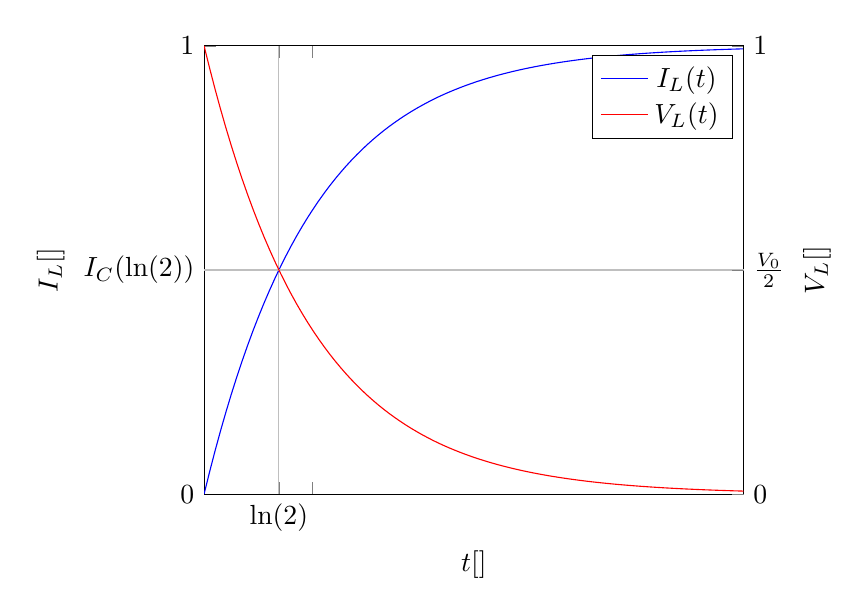
\begin{tikzpicture}
        \begin{axis}[
            axis y line*=left,
            xlabel = {\(t [\unit{\second}]\)},
            xticklabels={,,},
            ylabel = {\(I_L [\unit{\ampere}]\)},
            xmin = 0, xmax = 5,
            ymin = 0, ymax = 1,
            xtick = {0, 1}, ytick = {0, 1},
            extra tick style = {grid=major},
            extra x ticks = {ln(2)},
            extra x tick labels = {\(\ln(2)\)},
            extra y ticks = {0.5},
            extra y tick labels = {\(I_C(\ln(2))\)},
        ]
            \addplot[
            domain = 0:5,
            samples = 100,
            color = blue
            ]
            {1 - exp(-x)};
        \end{axis}

        \begin{axis}[
            axis y line*=right,
            axis x line = none,
            ylabel = {\(V_L [\unit{\volt}]\)},
            ylabel near ticks, yticklabel pos=right,
            xmin = 0, xmax = 5,
            ymin = 0, ymax = 1,
            xtick = {0, 1}, ytick = {0, 1},
            extra tick style = {grid=major},
            extra y ticks = {0.5},
            extra y tick labels = {\(\frac{V_0}{2}\)},
        ]
            \addlegendimage{color=blue}\addlegendentry{\(I_L(t)\)}
            \addplot[
            domain = 0:5,
            samples = 100,
            color = red
            ]
            {exp(-x)};
            \addlegendimage{color=red}\addlegendentry{\(V_L(t)\)}
        \end{axis}
    \end{tikzpicture}
\end{center}

\question{}

\begin{center}
    \begin{circuitikz}
        \draw (0, 2) to[V_={\qty{10}{\volt}}] (0, 0) node[ground]{};
        \draw (6, 0) node[ground]{} to[R, l=\qty{20}{\kilo\ohm}] (6, 2) to[R, l=\qty{20}{\kilo\ohm}] (4, 2) node[circ]{\(u_3\)} to[R, l=\qty{20}{\kilo\ohm}] (2, 2) node[circ]{\(u_2\)} to[R, l=\qty{20}{\kilo\ohm}] (0, 2) node[circ]{\(u_1\)};
        \draw (4, 2) to[R, l_=\qty{20}{\kilo\ohm}] (4, 0) node[ground]{};
        \draw (2, 2) to[R, l_=\qty{20}{\kilo\ohm}] (2, 0) node[ground]{};
        \draw (6, 2) to[short] (7, 2) node[ocirc]{\(u_4\)};
    \end{circuitikz}
\end{center}
Using nodal voltage analysis, we obtain the following equations:
\begin{align}
    u_1 &= \qty{10}{\volt} \\
    u_1 &= 3u_2 - u_3 \\
    u_2 &= 3u_3 - u_4 \\
    u_3 &= 2u_4
\end{align}
Solving for these gives us \(u_4 = \frac{1}{13} \qty{10}{\volt} \approx \qty{0.77}{\volt}\).
The Thévenin equivalent resistance is \(\frac{8}{13} \qty{20}{\kilo\ohm} \approx \qty{12.31}{\kilo\ohm}\).
The equivalent circuit is thus
\begin{center}
    \begin{circuitikz}
        \draw (0, 2) to[V, l=\(V_{th}\), a_={\qty{0.77}{\volt}}] (0, 0) node[ground]{};
        \draw (0, 2) to[R, l=\(R_{th}\), a=\qty{12.31}{\kilo\ohm}] (2, 2) to[R, l=\(R_L\), a=\qty{3}{\kilo\ohm}, i=\(i_L\)] (2, 0) node[ground]{};
    \end{circuitikz}
\end{center}
We find that \(i_L = \frac{V_{th}}{R_{th} + R_L} \approx \qty{5.03e-5}{\ampere}\).

\question{}

\begin{center}
    \begin{circuitikz}
        \draw (0, 2) to[V_=\qty{5}{\volt}] (0, 0) to[short] (6, 0) to[C, l={\(C = \qty{5}{\nano\farad}\)}, v<=\(V_C(t)\)] (6, 2) to[L, l={\(L = \qty{50}{\micro\henry}\)}, mirror, i<_=\(I_L(t)\)] (4, 2) to[R, l=\(R\), a=\qty{10}{\ohm}] (2, 2) to[opening switch, l=\(s_1\), mirror, invert] (0, 2);
        \draw (2, 2) to[switch, l=\(s_2\)] (2, 0);
        \draw (0, 0) node[ground]{};
    \end{circuitikz}
\end{center}
The initial conditions are \(V_C(0) = \qty{5}{\volt}\) and \(I_L(0) = \qty{0}{\ampere}\).
Performing nodal voltage analysis at \(t \geqslant 0\), we obtain the equations
\begin{align}
    I_L(t) &= C \dv{V_C}{t} \\
    -I_L(t) R - V_C(t) &= L \dv{I_L}{t}
\end{align}
Let \(x_1(t) = V_C(t)\) and \(x_2(t) = I_L(t)\).
In state space form, we get
\begin{equation}
    \dv{t} \bm{x}(t) =
    \begin{bmatrix}
        0 & \frac{1}{C} \\
        -\frac{1}{L} & -\frac{R}{L}
    \end{bmatrix} \bm{x}(t) =
    \underbrace{\begin{bmatrix}
        0 & \frac{1}{\num{5e-9}} \\
        -\frac{1}{\num{50e-6}} & -\frac{10}{\num{50e-6}}
    \end{bmatrix}}_{\bm{A}} \bm{x}(t)
\end{equation}
The eigenvalues are
\begin{align}
    \begin{vmatrix}
        -\lambda & \num{2e8} \\
        \num{-2e4} & \num{-2e5} - \lambda
    \end{vmatrix} &= \lambda^2 + (\num{2e5})\lambda + (\num{4e12}) = 0 \\
    \implies \lambda &= -10^5 \pm \sqrt{10^{10} - \num{4e12}} \\
    &= -10^5 \pm 10^5 \sqrt{1 - \num{4e2}} = -10^5 \pm 10^5 \sqrt{399} j \\
    &\approx -10^5 \pm (\num{2e6}) j
\end{align}
The eigenvectors are
\begin{align}
    \bm{A} - \lambda_1 \bm{I} &=
    \begin{bmatrix}
        10^5 - 10^5 \sqrt{399} j & \num{2e8} \\
        \num{-2e4} & \num{-2e5} + 10^5 - 10^5 \sqrt{399} j
    \end{bmatrix} \\
    &= \begin{bmatrix}
        10^5 - 10^5 \sqrt{399} j & \num{2e8} \\
        \num{-2e4} & -10^5 - 10^5 \sqrt{399} j
    \end{bmatrix} \\
    R_1 \leftarrow \frac{R_1}{-\lambda_1} &\implies \begin{bmatrix}
        1 & 5 + 5 \sqrt{399} j \\
        \num{-2e4} & -10^5 - 10^5 \sqrt{399} j
    \end{bmatrix} \\
    R_2 \leftarrow R_2 - (\num{2e4}) R_1 &\implies \begin{bmatrix}
        1 & 5 + 5 \sqrt{399} j \\
        0 & 0
    \end{bmatrix} \implies \bm{v}_1 =
    \begin{bmatrix}
        -5 - 5 \sqrt{399} j \\
        1
    \end{bmatrix} \approx
    \begin{bmatrix}
        -5 - 100j \\
        1
    \end{bmatrix} \\
    \bm{A} - \lambda_2 \bm{I} &=
    \begin{bmatrix}
        10^5 + 10^5 \sqrt{399} j & \num{2e8} \\
        \num{-2e4} & \num{-2e5} + 10^5 + 10^5 \sqrt{399} j
    \end{bmatrix} \\
    &= \begin{bmatrix}
        10^5 + 10^5 \sqrt{399} j & \num{2e8} \\
        \num{-2e4} & -10^5 + 10^5 \sqrt{399} j
    \end{bmatrix} \\
    R_1 \leftarrow \frac{R_1}{-\lambda_2} &\implies \begin{bmatrix}
        1 & 5 - 5 \sqrt{399} j \\
        \num{-2e4} & -10^5 + 10^5 \sqrt{399} j
    \end{bmatrix} \\
    R_2 \leftarrow R_2 + (\num{2e4}) R_1 &\implies \begin{bmatrix}
        1 & 5 - 5 \sqrt{399} j \\
        0 & 0
    \end{bmatrix} \implies \bm{v}_1 =
    \begin{bmatrix}
        -5 + 5 \sqrt{399} j \\
        1
    \end{bmatrix} \approx
    \begin{bmatrix}
        -5 + 100j \\
        1
    \end{bmatrix} \\
    \implies \bm{V} &\approx
    \begin{bmatrix}
        -5 - 100j & -5 + 100j \\
        1 & 1
    \end{bmatrix} \\
    \bm{V}^{-1} &\approx
    \frac{1}{200} \begin{bmatrix}
        j & 100 + 5j \\
        -j & 100 - 5j
    \end{bmatrix}
\end{align}
The transformed initial condition is
\begin{equation}
    \bm{z}(0) = \bm{V}^{-1}
    \begin{bmatrix}
        5 \\
        0
    \end{bmatrix} \approx
    \begin{bmatrix}
        \frac{j}{40} \\
        -\frac{j}{40}
    \end{bmatrix}
\end{equation}
Solving the diagonalized system, we have
\begin{equation}
    \dv{t} \bm{z}(t) =
    \begin{bmatrix}
        \lambda_1 & 0 \\
        0 & \lambda_2
    \end{bmatrix} \bm{z}(t) \implies \bm{z}(t) \approx
    \begin{bmatrix}
        \frac{j}{40} e^{(-10^5 + (\num{2e6}) j) t} \\
        -\frac{j}{40} e^{(-10^5 - (\num{2e6}) j) t}
    \end{bmatrix}
\end{equation}
The final equation is thus
\begin{align}
    \bm{x}(t) = \bm{V} \bm{z}(t) &\approx
    \frac{j}{40} \begin{bmatrix}
        -5 - 100j & -5 + 100j \\
        1 & 1
    \end{bmatrix}
    \begin{bmatrix}
        e^{(-10^5 + (\num{2e6}) j) t} \\
        -e^{(-10^5 - (\num{2e6}) j) t}
    \end{bmatrix} \\
    &= \frac{j}{40} \begin{bmatrix}
        -5 (e^{(-10^5 + (\num{2e6}) j) t} - e^{(-10^5 - (\num{2e6}) j) t}) \\
        e^{(-10^5 + (\num{2e6}) j) t} - e^{(-10^5 - (\num{2e6}) j) t}
    \end{bmatrix} \\
    &= \frac{je^{-10^5 t}}{40} \begin{bmatrix}
        -5 (e^{(\num{2e6}) j t} - e^{(\num{-2e6}) j t}) - 100j (e^{(\num{2e6}) j t} + e^{(\num{-2e6}) j t}) \\
        e^{(\num{2e6}) j t} - e^{(\num{-2e6}) j t}
    \end{bmatrix} \\
    &= \frac{je^{-10^5 t}}{40} \begin{bmatrix}
        -10j \sin((\num{2e6}) t) - 200j \cos((\num{2e6}) t) \\
        2j \sin((\num{2e6}) t)
    \end{bmatrix} \\
    &= \frac{e^{-10^5 t}}{40} \begin{bmatrix}
        10 \sin((\num{2e6}) t) + 200 \cos((\num{2e6}) t) \\
        -2 \sin((\num{2e6}) t)
    \end{bmatrix}
\end{align}

\end{document}
